\documentclass[a5paper,11pt]{book}
\usepackage{geometry}

\usepackage[T1]{fontenc}
\usepackage{fancyhdr}

\usepackage{amsmath}
\usepackage{amsthm}
\usepackage{amssymb}
\usepackage[spanish,es-nodecimaldot]{babel}

\usepackage{float}

\usepackage{hyperref}
\usepackage{graphicx}

\usepackage{listings}
\usepackage{xcolor}

\usepackage{thmtools}
\usepackage[framemethod=TikZ]{mdframed}
\mdfsetup{skipabove=1em,skipbelow=0em, innertopmargin=5pt, innerbottommargin=6pt}

\theoremstyle{definition}

\makeatletter

\declaretheoremstyle[headfont=\bfseries\sffamily, bodyfont=\normalfont, mdframed={ nobreak } ]{thmgreenbox}
\declaretheoremstyle[headfont=\bfseries\sffamily, bodyfont=\normalfont, mdframed={ nobreak } ]{thmredbox}
\declaretheoremstyle[headfont=\bfseries\sffamily, bodyfont=\normalfont]{thmbluebox}
\declaretheoremstyle[headfont=\bfseries\sffamily, bodyfont=\normalfont]{thmblueline}
\declaretheoremstyle[headfont=\bfseries\sffamily, bodyfont=\normalfont, numbered=no, mdframed={ rightline=false, topline=false, bottomline=false, }, qed=\qedsymbol ]{thmproofbox}
\declaretheoremstyle[headfont=\bfseries\sffamily, bodyfont=\normalfont, numbered=no, mdframed={ nobreak, rightline=false, topline=false, bottomline=false } ]{thmexplanationbox}


\declaretheorem[numberwithin=chapter, style=thmgreenbox, name=Definición]{definition}
\declaretheorem[sibling=definition, style=thmredbox, name=Corolario]{corollary}
\declaretheorem[sibling=definition, style=thmredbox, name=Proposición]{prop}
\declaretheorem[sibling=definition, style=thmredbox, name=Teorema]{theorem}
\declaretheorem[sibling=definition, style=thmredbox, name=Lema]{lemma}


\declaretheorem[numbered=no, style=thmexplanationbox, name=Explicación]{explanation}
\declaretheorem[numbered=no, style=thmproofbox, name=Demostración]{replacementproof}
\declaretheorem[style=thmbluebox, name=Ejercicio]{ex}
\declaretheorem[style=thmbluebox,  numbered=no, name=Ejemplo]{eg}
\declaretheorem[style=thmblueline, numbered=no, name=Nota]{note}

\renewenvironment{proof}[1][\proofname]{\begin{replacementproof}}{\end{replacementproof}}

\AtEndEnvironment{eg}{\null\hfill$\diamond$}%

\newtheorem*{notation}{Notación}
\newtheorem*{previouslyseen}{Como ya se ha visto}
\newtheorem*{problem}{Problema}
\newtheorem*{solution}{Solución}
\newtheorem*{observe}{Observe}
\newtheorem*{property}{Propiedad}

% Colores flexoki
\definecolor{bgcolor}{RGB}{255, 252, 240}
\definecolor{txcolor}{RGB}{16, 15, 15}
\definecolor{tx2color}{RGB}{111, 110, 105}
\definecolor{grcolor}{RGB}{102, 128, 11}
\definecolor{recolor}{RGB}{175, 48, 41}
\definecolor{cycolor}{RGB}{36, 131, 123}

% Para poner acentos en código
\lstset{literate=
  {á}{{\'a}}1 {é}{{\'e}}1 {í}{{\'i}}1 {ó}{{\'o}}1 {ú}{{\'u}}1
  {Á}{{\'A}}1 {É}{{\'E}}1 {Í}{{\'I}}1 {Ó}{{\'O}}1 {Ú}{{\'U}}1
  {à}{{\`a}}1 {è}{{\`e}}1 {ì}{{\`i}}1 {ò}{{\`o}}1 {ù}{{\`u}}1
  {À}{{\`A}}1 {È}{{\`E}}1 {Ì}{{\`I}}1 {Ò}{{\`O}}1 {Ù}{{\`U}}1
  {ä}{{\"a}}1 {ë}{{\"e}}1 {ï}{{\"i}}1 {ö}{{\"o}}1 {ü}{{\"u}}1
  {Ä}{{\"A}}1 {Ë}{{\"E}}1 {Ï}{{\"I}}1 {Ö}{{\"O}}1 {Ü}{{\"U}}1
  {â}{{\^a}}1 {ê}{{\^e}}1 {î}{{\^i}}1 {ô}{{\^o}}1 {û}{{\^u}}1
  {Â}{{\^A}}1 {Ê}{{\^E}}1 {Î}{{\^I}}1 {Ô}{{\^O}}1 {Û}{{\^U}}1
  {ã}{{\~a}}1 {ẽ}{{\~e}}1 {ĩ}{{\~i}}1 {õ}{{\~o}}1 {ũ}{{\~u}}1
  {Ã}{{\~A}}1 {Ẽ}{{\~E}}1 {Ĩ}{{\~I}}1 {Õ}{{\~O}}1 {Ũ}{{\~U}}1
  {œ}{{\oe}}1 {Œ}{{\OE}}1 {æ}{{\ae}}1 {Æ}{{\AE}}1 {ß}{{\ss}}1
  {ű}{{\H{u}}}1 {Ű}{{\H{U}}}1 {ő}{{\H{o}}}1 {Ő}{{\H{O}}}1
  {ç}{{\c c}}1 {Ç}{{\c C}}1 {ø}{{\o}}1 {Ø}{{\O}}1 {å}{{\r a}}1 {Å}{{\r A}}1
  {€}{{\euro}}1 {£}{{\pounds}}1 {«}{{\guillemotleft}}1
  {»}{{\guillemotright}}1 {ñ}{{\~n}}1 {Ñ}{{\~N}}1 {¿}{{?`}}1 {¡}{{!`}}1 
}


%Code listing style named "mystyle"
\lstdefinestyle{mystyle}{
  backgroundcolor=\color{bgcolor},
  commentstyle=\color{tx2color},
  keywordstyle=\color{recolor},
  numberstyle=\ttfamily\color{txcolor},
  stringstyle=\color{grcolor},
  identifierstyle=\color{cycolor},
  basicstyle=\ttfamily\footnotesize,
  breakatwhitespace=false,
  breaklines=true,
  captionpos=b,
  keepspaces=true,
  numbers=left,
  numbersep=5pt,
  showspaces=false,
  showstringspaces=false,
  showtabs=true,
  tabsize=4,
}

%"mystyle" code listing set
\lstset{style=mystyle}

\renewcommand\qedsymbol{$\blacksquare$}

% 'dedication' environment: To add a dedication paragraph at the start of book
% Source: http://www.tug.org/pipermail/texhax/2010-June/015184.html
\newenvironment{dedication}
{
    \cleardoublepage
    \thispagestyle{empty}
    \vspace*{\stretch{1}}
    \hfill\begin{minipage}[t]{0.66\textwidth}
        \raggedright
    }
    {
    \end{minipage}
    \vspace*{\stretch{3}}
    \clearpage
}

% Chapter quote at the start of chapter
% Source: http://tex.stackexchange.com/a/53380
\makeatletter
\newenvironment{chapquote}[2][2em]
{\setlength{\@tempdima}{#1}%
    \def\chapquote@author{#2}%
    \parshape 1 \@tempdima \dimexpr\textwidth-2\@tempdima\relax%
\itshape}
{\par\normalfont\hfill--\ \chapquote@author\hspace*{\@tempdima}\par\bigskip}
\makeatother


\title{\textbf{Notas de Análisis Numérico} \\ \small con Lozano :) }
\author{Francisco Galindo}

\date{Última actualización: \today}

\begin{document}
\frontmatter

\maketitle

\begin{dedication}
    Para Yael y el Erick
\end{dedication}

\tableofcontents
\listoffigures
\listoftables


\mainmatter

\chapter{Introducción}

\begin{chapquote}{Lozano, 2024}
    ``[...] En ese sentido, el análisis numérico es como el Fortnite.''
\end{chapquote}


\section{Sobre raíces de polinomios}

Prescindiendo del grado, todo polinomio tiene asociado un grupo, y
descubrió que:

\begin{quote}
    Una ecuación es soluble si y solo si, su grupo de Galois es soluble,
    entendido por ecuación soluble aquella que puede resolverse mediante
    operaciones elementales con radicales
\end{quote}

Lo anterior se logró mediante la observación del grupo de permutaciones
de \(n\) elementos, es decir \(S_n\). Él se dio cuenta de que el primer
grupo sin soluciones es \(S_5\), por lo que ningún polinomio de grado
mayor o igual a 5 tiene una solución exacta mediante operaciones
simples.

\section{Métodos de solución de problemas}

\subsection{Métodos analíticos (exactos)}

Se trata de los métodos que permiten encontrar una solución en forma de
fórmula, permiten calcular una cantidad en función de otra. Por ejemplo:

\begin{equation*}{
        ax^2 + bx + c = 0 \implies x = \frac{-b \pm \sqrt{b^2 -4ac}}{2a}
}\end{equation*}

\subsection{Soluciones gráficas (cualitativas)}

Se utilizan para aproximar una solución de manera visual. No son precisas, pero
son fáciles de usar. Si se quieren encontrar las raíces de la siguiente
ecuación:

\begin{equation}\label{primer-problema}
        x^2 - 4 - sin(x) = 0
\end{equation}

A primera vista no resulta posible (no lo es) hacer despejes para
encontrar los valores de \(x\) que satisfacen la ecuación. Sin embargo,
si se escribe de la siguiente manera:

\begin{equation*}{
        \underbrace{x^2 - 4}_{f(x)} = \underbrace{sin(x)}_{g(x)}
}\end{equation*}

Lo anterior permite tener una idea intuitiva de las raíces como las
intersecciones entre las gráficas de las funciones \(f(x)\) y \(g(x)\):

\begin{figure}[H]
    \centering
    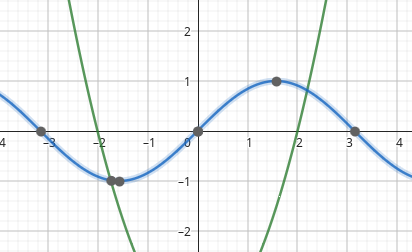
\includegraphics[width=1.0\textwidth]{img/papu.png}
    \caption{Visualización de soluciones por el método gráfico}
\end{figure}

Puede notarse así que las soluciones de la ecuación son:

\begin{equation*}{
        x \approx -1.8
}\end{equation*}

\begin{equation*}{
        x \approx 2.1
}\end{equation*}

\subsection{Métodos numéricos}

Son aproximaciones a soluciones de un problema. Generalmente se basa en
la conversión del problema original utilizando operaciones aritméticas
básicas. En teoría, el resultado es tan bueno como se desee. Para el
ejemplo anterior, usando \emph{GNU Octave}, los resultados son:

\begin{equation*}{
        x \approx -1.7360
}\end{equation*}

\begin{equation*}{
        x \approx 2.1937
}\end{equation*}

\section{Exactitud y error}

¿Qué tan buenas son las soluciones obtenidas anteriormente? Para
responder esta pregunta, es importante conocer ciertas definiciones
utilizadas durante el curso.

\begin{definition}[Exactitud]
    Es el grado de proximidad de una solución para un problema dado.


\end{definition}

\begin{eg}
    Un ejemplo es esta secuencia de aproximaciones progresivamente más exactas:

    \begin{align*} 
        \pi &\approx 3 \\ 
            &\approx 3.1 \\ 
            &\approx 3.14 \\ 
            &\approx 3.141592 \\ 
    \end{align*}

\end{eg}

\begin{definition}[Precisión]
    Es la medida que indica qué tan agrupados están los valores calculados a
    su valor real. La precisión se cuantifica mediante el número de
    \emph{cifras significativas}\footnote{Las cifras significativas son
    aquellas de las que se tiene certeza en los cálculos experimentales.}
\end{definition}


\section{Tipos de errores}

Al realizar procesos numéricos, es necesario determinar una condición de
parada, un \emph{threshold} para cuando el resultado sea exacto con
cierta precisión. Los siguientes conceptos serán útiles para denotar
estas condiciones de detención:

\begin{itemize}
    \item
        \textbf{Error absoluto}: Es la diferencia entre el valor real y el
        valor calculado. Generalmente tiene unidades físicas:

        \begin{equation*}{
                E_T = \text{Valor}_{\text{real}} - \text{Valor}_{\text{calculado}}
        }\end{equation*}
    \item
        \textbf{Error relativo (porcentual)}: Es la medida del error absoluto
        en términos porcentuales:

        \begin{equation*}{
                \varepsilon_{T} = \left| {\frac{E_T}{\text{Valor}_{\text{real}}}} \right| * 100 \%
        }\end{equation*}
\end{itemize}


\begin{ex}

    En un vertedero local se reciben camiones de desechos. Por lo general,
    en estos lugares, se pesan tales camiones en básculas. Suponiendo que
    hay dos básculas y una está recién calibrada, se pesa un camión, dando
    como resultado las siguientes mediciones:

    \begin{eqnarray*}
        P_{B_1} &= 3552\text{ kg}\\
        P_{B_2} &= 3633\text{ kg}
    \end{eqnarray*}

    Suponiendo que la báscula 1 (\(B_1\)) es la calibrada, ¿cuál es el error
    absoluto y relativo de la segunda báscula?

    \begin{solution}
        Para calcular el error, se utiliza:

        \begin{equation*}{
                E_T = P_{B_1} - P_{B_2} = 3552 - 3633 = -81 \text{ kg}
        }\end{equation*}

        Para calcular el error relativo, se usa:

        \begin{center}
            \boxed{\varepsilon_T = \left| \frac{P_{B_1} - P_{B)_2}}{P_{B_1}} \right| * 100\% = 2.28\%}
        \end{center}

    \end{solution}


\end{ex}


\section{Series de Taylor}

La serie de Taylor tiene múltiples aplicaciones en el área teórica y
aplicada, dentro de donde destacan las siguientes:

\begin{itemize}
    \item
        Aproximar una función mediante una serie de potencias
    \item
        Linearizar ecuaciones diferenciales o integrales
    \item
        Solucionar Ecuaciones Diferenciales no lineales alrededor de un punto
        de interés
    \item
        Resolución de integrales definidas
\end{itemize}

\begin{definition}[Serie de Taylor]

    En su versión de una sola variable, la serie de Taylor de la función $f$,
    con centro en $a$, es la siguiente:

    \begin{align*}
        f(x) &= f(a) + \frac{f'(a)}{1!}(x - a) + \frac{f''(a)}{2!}(x - a)^2 + ... \\
             &= \sum_{k = 0}^{\infty} \frac{f^{(k)}(a)}{k!}(x - a)^k
    \end{align*}

\end{definition}


\begin{ex}
    Obtenga la serie de Taylor de la función \(f(x) = e^x\) alrededor de \(x = 0\)
\end{ex}

\begin{solution}

    Empleando directamente la definición de una serie de Taylor, con \(a = 0\):
    \begin{equation*}{
            e^x = e^0 + \left[\frac{de^x}{dx}\right]_{x = 0} x + \left[\frac{d^2e^x}{dx^2}\right]_{x = 0} \frac{x^2}{2!} + \left[\frac{d^3e^x}{dx^3}\right]_{x = 0} \frac{x^3}{3!} + ...
    }\end{equation*}

    Simplificando:

    \begin{equation*}{
            \boxed{e^x = 1 + x + \frac{x^2}{2!} + \frac{x^3}{3!} + ...}
    }\end{equation*}

\end{solution}

\begin{ex}

    Considere el péndulo representado por la figura \ref{fig:pendulo}, donde
    las únicas fuerzas actuando son la tensión de la cuerda y el peso del
    péndulo. Para escribir la posición angular del péndulo como una función del
    tiempo, uno puede apoyarse en la Segunda Ley de Newton:

    \begin{figure}
        \centering
        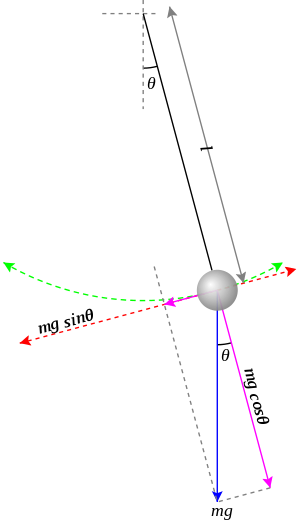
\includegraphics[height=3in]{img/pendulo.png}
        \caption{Diagrama de fuerzas de un péndulo simple.}
        \label{fig:pendulo}
    \end{figure}

    \begin{equation*}
        F = ma
    \end{equation*}

    Como el movimiento está restringido a una trayectoria circular, sólo es de
    interés el componente de la fuerza que es tangencial al movimiento del
    péndulo (el signo es negativo porque el ángulo siempre tiene signo
    contrario al vector de fuerza en este sistema de referencia):

    \begin{align*}
        F &= -mg \sin \theta\\
        a &= -g \sin \theta\\
    \end{align*}

    Considerando la siguiente relación entre la aceleración tangencial $a$ y la aceleración angular $\alpha$, donde $l$ es la longitud del péndulo:

    \begin{equation*}
        \alpha = \frac{a}{l}
    \end{equation*}

    Puede llegarse a la siguiente ecuación diferencial:

    \begin{align*}
        l \alpha &= -g \sin \theta\\
        \alpha &= -\frac{g}{l} \sin \theta \\
        \frac{d^2 \theta}{dt^2} &= -\frac{g}{l} \sin \theta \\
        0 &= \frac{d^2 \theta}{dt^2} + \frac{g}{l} \sin \theta
    \end{align*}

    Suponiendo que el péndulo oscila en ángulos pequeños (por ejemplo, que
    inicia desde el reposo con un ángulo de $\frac{\pi}{20}$), resuelva la
    siguiente ecuación diferencial:

    \begin{equation*}{
            \frac{d^2 \theta}{dt^2} + \frac{g}{l} \sin \theta = 0,
            \begin{cases}
                \theta(0) = \frac{\pi}{20}\\
                \theta'(0) = 0
            \end{cases}
    }\end{equation*}

    \begin{solution}

        La ecuación anterior tiene únicamente solución analítica mediante
        integrales elípticas (es necesario usar la serie del binomio). Sin
        embargo, como la oscilación inicial es pequeña, se puede aproximar el
        seno mediante series de Taylor.

        La serie de Taylor de la función seno, con centro en 0, es la siguiente:

        \begin{align*}
            \sin \theta &= \theta - \frac{\theta^3}{3!} + \frac{\theta^5}{5!} - \frac{\theta^7}{7!} + ... \\  
                        &= \theta \underbrace{- \frac{\theta^3}{6} + \frac{\theta^5}{120} - \frac{\theta^7}{5040} + ...}_{\text{despreciables cuando } \theta \text{ es pequeño}} \\
                        &\approx \theta
        \end{align*}

        Podemos concluir que, si el ángulo de oscilación es pequeño:

        \begin{equation*}{
                \sin \theta \approx \theta
        }\end{equation*}

        Sustituyendo, se obtiene la versión linearizada de la ecuación
        diferencial:

        \begin{equation*}{
                \frac{d^2 \theta}{dt^2} + \frac{g}{l} \theta = 0,
                \begin{cases}
                    \theta(0) = \frac{\pi}{20}\\
                    \theta'(0) = 0
                \end{cases}
        }\end{equation*}

        La solución analítica de la ecuación anterior es:

        \begin{equation*}{
                \boxed{\theta_{\text{lineal}} = \frac{1}{20} \pi \cos(\sqrt{\frac{g}{l}} t)}
        }\end{equation*}

    \end{solution}

    Si se compara la solución lineal con la no lineal, es posible
    observar que la aproximación es bastante acertada:

    \begin{figure}[H]
        \centering
        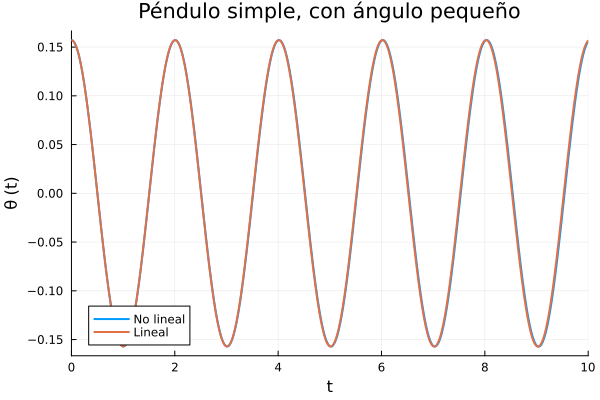
\includegraphics[width=1.0\textwidth]{img/small.png}
        \caption{Comparación de soluciones para $\theta(0) = \frac{\pi}{20}$}
        \label{fig:pendulo_sol_small}
    \end{figure}

    Sin embargo, para valores iniciales de $\theta$ más grandes, el error se
    vuelve evidente:

    \begin{figure}[H]
        \centering
        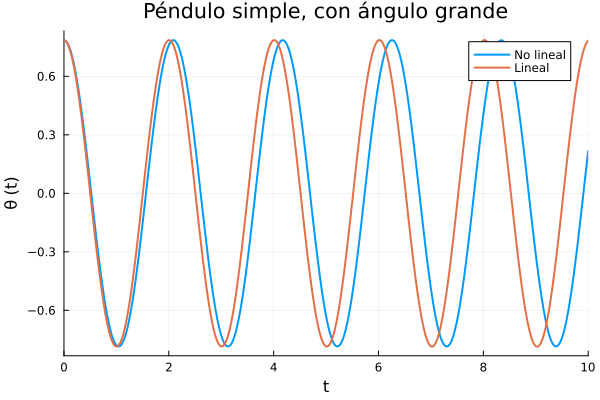
\includegraphics[width=1.0\textwidth]{img/big.png}
        \caption{Comparación de soluciones para $\theta(0) = \frac{\pi}{4}$}
        \label{fig:pendulo_sol_big}
    \end{figure}


\end{ex}


\begin{ex}[Aproximación de una integral definida mediante series de Taylor]

	En ocasiones, no es posible obtener la solución analítica exacta de
	ciertas integrales, ya sea porque no existe un método o requiere de
	tópicos más avanzados. Por ejemplo, supóngase que se tiene la siguiente
	integral \footnote{ Resulta que esta integral sí tiene solución
	analítica: 
		\begin{equation*}
		I = \left[Si(e^{x^2})\right]_{x=0}^{x=0.1}
		\end{equation*}
	}

	\begin{equation}\label{ex4:1}
		I = \int_{0}^{0.1} x \sin(e^{x^2}) dx
	\end{equation}

	\begin{solution}

	El término exponencial dentro del seno dificulta mucho la resolución de
	la integral propuesta. A pesar de todo, puede utilizarse la serie de
	Taylor de la función seno:

	\begin{equation*}
		\sin u = \sum_{n = 0}^{\infty} \frac{(-1)^n}{(2n + 1)!} u^{2n +
		1}
	\end{equation*}

	Empleando esta serie dentro de \ref{ex4:1}:

	\begin{align*}
		I &= \int_{0}^{0.1} x \sin(e^{x^2}) dx \\
		%
		  &= \int_{0}^{0.1} x \sum_{n = 0}^{\infty} \frac{(-1)^n}{(2n +
		  1)!} (e^{x^2})^{2n + 1} dx \\
		  %
		  &= \int_{0}^{0.1} x \sum_{n = 0}^{\infty} \frac{(-1)^n}{(2n +
		  1)!} e^{x^2(2n + 1)} dx \\
		  %
		  &= \sum_{n = 0}^{\infty} \int_{0}^{0.1} \frac{(-1)^n}{(2n +
		  1)!} x e^{x^2(2n + 1)} dx \\
		  %
		  &= \sum_{n = 0}^{\infty} \int_{0}^{0.1} \frac{(-1)^n}{(2n +
		  1)!} x e^{x^2(2n + 1)} dx \\
		  %
		  &= \sum_{n = 0}^{\infty} \frac{(-1)^n}{(2n + 1)!}
		  \int_{0}^{0.1} x e^{x^2(2n + 1)} dx \\
	\end{align*}

	Si se hace el cambio de variable $u = (2n + 1) x^2$, $du = 2(2n + 1)x dx$:

	\begin{align*}
		I &= \sum_{n = 0}^{\infty} \frac{(-1)^n}{2(2n + 1)(2n + 1)!}
		  \int_{0}^{0.1} 2(2n + 1) x e^{x^2(2n + 1)} dx \\
		  %
		  &= \sum_{n = 0}^{\infty} \frac{(-1)^n}{2(2n + 1)(2n + 1)!}
		  \left[e^{2n + 1}x^2 \right]_{0}^{0.1}\\
		  %
		  &= \sum_{n = 0}^{\infty} \frac{(-1)^n}{2(2n + 1)(2n + 1)!}
		  \left[e^{0.1(2n + 1)} - 1 \right]\\
		  %
		  &= \frac{1}{2} \sum_{n = 0}^{\infty} \frac{(-1)^n}{(2n + 1)(2n
		  + 1)!} \left[e^{0.1(2n + 1)} - 1 \right]\\
	\end{align*}

	En resumen, el resultado es el siguiente:

	\begin{equation*}
		\int_{0}^{0.1} x \sin(e^{x^2}) dx = \frac{1}{2} \sum_{n = 0}^{\infty} \frac{(-1)^n}{(2n + 1)(2n + 1)!} \left[e^{0.1(2n + 1)} - 1 \right]
	\end{equation*}



	Evaluando con cuatro términos en
	\emph{Mathematica} usando \emph{NIntegrate}, el resultado es:

	\begin{align*}
		\int_{0}^{0.1} x \sin(e^{x^2}) dx &\approx \frac{1}{2} \sum_{n = 0}^{3} \frac{(-1)^n}{(2n + 1)(2n + 1)!} \left[e^{0.1(2n + 1)} - 1 \right]\\
						  &\approx 0.00422084
	\end{align*}

	Puede compararse este resultado con la solución analítica:
	%falta comparación con solución numérica de wolfram

	\begin{center}
		\boxed{\int_{0}^{0.1} x \sin(e^{x^2}) dx \approx 0.00422084}
	\end{center}

	De los resultados anteriores puede concluirse que la aproximación
	semi-analítica es aceptable.
	\end{solution}

\end{ex}

\begin{ex}[Determinación del orden de aproximación de un método numérico]

	Es necesario definir la derivada:

	\begin{definition}[La derivada]
		La definición formal de derivada de una función de una variable $f$ es
		la siguiente:

		\begin{equation}\label{eqn:def-derivada}
			\frac{df}{dx} = \lim_{h \rightarrow 0} \frac{f(x + h) - f(x)}{h}
		\end{equation}

	\end{definition}
	A partir de \ref{eqn:def-derivada}, puede aproximarse la derivada de la
	siguiente manera:

	\begin{equation*}
		\frac{df}{dx} \approx \frac{f(x + h) - f(x)}{h}
	\end{equation*}

	Las aproximaciones mejoran conforme $h \rightarrow 0$. Sin embargo, no
	dice nada de la forma en que decrece. Uno de los usos más portentosos de
	la serie de Taylor es la obtención es la obtención de esquemas de
	derivación de orden $n$, además de obtener un término que cuantifica el
	orden del error. En el caso de la serie de Taylor truncada hasta el
	término de primer orden:

	\begin{equation*}
		f(x) = f(a) + f'(a)(x-a) + O(x-a)^2
	\end{equation*}

	$O$ indica el orden de magnitud de los términos que se desprecian. Si
	$h = x - a$:

	\begin{equation*}
		f(a + h) = f(a) + f'(a)h + O(h^2)
	\end{equation*}

	Precisamente, de esta ecuación se pude despejar la primera derivada:

	\begin{equation*}
		f'(a) = \frac{f(a + h) - f(a)}{h} + \overbrace{O(h)}^{O(h^2)/h}
	\end{equation*}

	Sabiendo esto, obtenga la derivada evaluada en $x = 2$ de la función:

	\begin{equation*}
		f(x) = 3x^2 + 2e^{-3x} + \sin x
	\end{equation*}

	Sabiendo que el valor exacto de la derivada es

	\begin{equation*}
		f'(2) =11.56898065039286
	\end{equation*}

	Calcule la derivada numérica haciendo progresivamente pequeño a $h$.
	Obtenga una gráfica $\log h - \log \varepsilon_T$.

	\begin{solution}[Mediante un programa de Fortran]

		El siguiente código evalúa la derivada con diferencias finitas:

		\lstinputlisting[language=Fortran]{./programas/derivada-diferencias-finitas/derivada-simple.f90}

		Si se quiere mejorar poco a poco la aproximación, puede
		utilizarse un ciclo:

		\lstinputlisting[language=Fortran, caption=Programa que aproxima
		la derivada mediante diferencias finitas cada vez menores.,
		label={lst:derivada_logh_logepsilon}]{./programas/derivada-diferencias-finitas/derivada_logh_logepsilon.f90}

		A partir del código dado en \ref{lst:derivada_logh_logepsilon},
		iterando de manera que $h$ se volviera más pequeña, pudo hacerse
		una aproximación cada vez mejor de $f'(2)$

	\end{solution}
\end{ex}

\section{Aproximación de errores con serie de Taylor}

Cuando se desarrollan experimentos, necesariamente existen incertidumbres, o
sea, errores inevitables que aparecen de la medición con instrumentos. Para
aproximar cómo las incertidumbres perturban las mediciones físicas, las series
de Taylor multivariables resultan de gran utilidad.

\begin{definition}[Serie de Taylor multivariable]

	La serie de Taylor de varias variables para una función $f$ que depende
	de las variables $\overline{x} = (x_1, x_2, ..., x_n)$, alrededor del
	punto $ \overline{a} = (a_1, a_2, ..., a_n)$ es:

	\begin{align*}
		f = & \ f(x_1, x_2, ..., x_n) = f(a_1, a_2, ..., a_n) + \\ 
		    & + \sum_{k=1}^{n} \
		    \frac{\partial f(a_1,a_2,...,a_n)}{\partial x_k}(x_k-a_k)\\
		    & + \frac{1}{2!} \sum_{j=1}^{n} \sum_{k=1}^{n} \
		    \frac{\partial^2 f(a_1,a_2,...,a_n)}{\partial x_k \partial
		    x_j}(x_k-a_k)(x_j-a_j)\\
		    & + ...
	\end{align*}
	\label{eq:def-taylor-multi}

\end{definition}

A partir de la definición \ref{eq:def-taylor-multi}, puede estimarse la
incertidumbre en una función multivariable. Si asumimos que el punto $(a_1, a_2,
..., a_n)$ está cerca de $(x_1, x_2, ..., x_n)$, es decir:

\begin{align*}
    x_1 - a_1 &< 1 \\
    x_2 - a_2 &< 1 \\
              &\vdots \\
    x_n - a_n &< 1
\end{align*}

Puede simplificarse \ref{eq:def-taylor-multi} a sus términos de primer orden:

\begin{align*}
	f(\overline{x}) \approx f(\overline{a}) + \sum_{k=1}^{n} \
		\frac{\partial f(\overline{a})}{\partial x_k} (x_k - a_k) \\
	f(\overline{x}) - f(\overline{a}) \approx \sum_{k=1}^{n} \
		\frac{\partial f(\overline{a})}{\partial x_k} (x_k - a_k)
\end{align*}

Tomando el valor absoluto en ambos lados \footnote{Aquí se utiliza la
desigualdad del Minkowski: $|a_1 + a_2 + ... + a_3| \leq |a_1| + |a_2| + ... +
|a_n|$. En el caso de dos términos, a esta desigualdad se le llama
\textit{desigualdad del triángulo}.}:

\begin{equation} \label{eq:desigualdad-tri-taylor}
	\Delta f \leq \sum_{k=1}^{n} \left |\ 
		\frac{\partial f(\overline{a})}{\partial x_k} \right| \
		\Delta x_k
\end{equation}

Es la ecuación \ref{eq:desigualdad-tri-taylor} la que proporcionará las
incertidumbres de cada una de las variables $x_i\ \forall i \in N, i \leq n$.

\begin{ex}

	Suponga que una resistencia eléctrica que se usa para calentar agua se
	alimenta a un contacto de 127 [V] y consume una corriente eléctrica de
	2[A] (datos obtenidos con un multímetro). Si el equipo de medición
	indica que el voltaje tiene una incertidumbre de $\pm$ 0.3 [V] t la
	corriente $\pm$ 0.1 [A], ¿Cuál es la incertidumbre total de la medición de
	la potencia?

	\begin{solution}
		La potencia eléctrica que disipa un dispositivo eléctrico se
		calcula mediante la siguiente expresión:

		\begin{equation*}
			P = IV
		\end{equation*}

		La incertidumbre se calcula con la misma expresión,
		escribiéndolo de manera explícita:

		\begin{equation*}
			P(I, V) = IV
		\end{equation*}

		Y, según el enunciado:

		\begin{align*}
			\Delta V &= 0.3 \text{ [V]} \\
			\Delta I &= 0.1 \text{ [A]}
		\end{align*}


		Aplicando la ecuación \ref{eq:desigualdad-tri-taylor},

		\begin{align*}
			\Delta P &\leq
			\left| \frac{\partial P}{\partial I} \right| \Delta I +
			\left| \frac{\partial P}{\partial V} \right| \Delta V \\
				 &\leq \left| V \right| \Delta I + \left| I\right|
				 \Delta V \\
				 &\leq 127 [V](0.1 [I]) + 2 [I](0.3 [V]) \\
			\therefore \Delta P &\leq 13.3 [W]
		\end{align*}
	\end{solution}
\end{ex}


\begin{ex}
	
	Se desea determinar la energía cinética de una partícula, la cual se
	calcula con la siguiente expresión:

	\begin{equation*}
		E = \frac{1}{2} m v^2
	\end{equation*}

	Si se ha determinado de manera experimental que \(m = 10^{-8}\) [kg] y $v
	= 15 [\frac{m}{s}]$, determine la energía cinética si la incertidumbre
	de las medidas para la masa y la velocidad son de $\pm 10^{-10}$ [kg] y
	$\pm 0.02 [\frac{m}{s}]$.

	\begin{solution}

		Sustituyendo directamente sin las incertidumbre, la energía
		cinética es:

		\begin{equation*}
			E = 1.125 \times 10^{-6} \text{ [J]}
		\end{equation*}

		La función cuya incertidumbre se quiere encontrar es

		\begin{equation*}
			E(m, v) = \frac{1}{2} m v^2
		\end{equation*}

		La ecuación \ref{eq:desigualdad-tri-taylor} permite calcular la
		incertidumbre:

		\begin{align*}
			\Delta E &\leq \left[ \left| \frac{\partial E}{\partial m}
			\right| \Delta m + \left| \frac{\partial E}{\partial v}
		\right| \Delta d \right]_{m = 10^{-8}, v = 15}\\
		%
				 &\leq \left[ \left| \frac{v^2}{2}
			\right| \Delta m + \left| m v \right| \Delta d 
		\right]_{m = 10^{-8}, v = 15} \\
		%
				 &\leq 1.425 \times 10^{-8} \text{ [J]}
		\end{align*}

		Así, la energía cinética es

		\begin{center}
			\boxed{E(m, v) = 1.125
			\times 10^{-6} \pm 1.425 \times 10^{-8} \text{ [J]}}
		\end{center}

	\end{solution}
\end{ex}

\chapter{Conceptos de Fortran 90}

\begin{chapquote}{El Erick, 2024}
    ``Tú no usas Fortran, ¿verdad? Tú sí eres inteligente.''
\end{chapquote}

\section{Fortran apesta}

\begin{itemize}
	\item{El lenguaje no distingue mayúsculas de minúsculas.}
	\item{Por defecto, las variables que
			\begin{itemize}
				\item{inician con $i$, $j$, $k$, $l$, $m$ son enteras}
				\item{y el resto de letras son reales.}
			\end{itemize}
		}
	\item{El código que escribamos siempre tendrá estructura modular y
			jerárquica:
			\begin{itemize}
				\item{Programas}
				\item{Subrutinas}
				\item{Funciones}
			\end{itemize}
		}
	\item{El código siempre se ejecutará de izquierda a derecha y de arriba
		a abajo.}
\end{itemize}

\section{Sintaxis del lenguaje}

\begin{itemize}
	\item{\texttt{IMPLICIT NONE}: elimina la asignación por defecto de los enteros. Causa errores y advertencias cuando una variable no sea usada}
	\item{\texttt{OPEN(UNIT, FILE, STATUS, ERR)}: }
\end{itemize}


\end{document}
